%
\section{Apex Coordinates}\label{cap:apex_coord}
%
The apex and modified apex coordinate system is described in \cite{rich95}. The
apex latitude $\lambda_A$ is constant along a field line with an apex height
$h_A$. 
%
\begin{equation}
    \lambda_A = \pm cos^{-1} (1+\frac{h_A}{R_{eq}})^{-1/2}
\end{equation}
%
with $R_{eq}$ denoting the Earth radius at the equator and the 
$\pm$ sign for the location of the field line foot point in the
northern / southern  geomagnetic hemisphere. In the electrodynamo part of TIEGCM
modified apex coordinates are used. Modified apex coordinates $\lambda_m$ 
have a reference height $h_R$ associated with them.
%
\begin{equation}
    \lambda_m = \pm cos^{-1} \bigl( \frac{R_E + h_R}{R_E + h_A} \bigr)^{-1/2}
\end{equation}
%
The mean Earth radius is denoted by $R_E$ assuming a spherical Earth.
The reference height $h_R$ is assumed to be the bottom boundary of the ionosphere 
at $h_R = h_0 = 90 km$.
One of the advantages for using modified apex
latitudes $\lambda_m$ is that the field line foot point latitudes are 
continuous at the 90 km (for TIEGCM) lower boundary
of the model. Apex latitudes, in contrast, would have a gap at low
latitudes since only field line with an apex of at least 90 km could be used for 
the field line integration. 
The apex longitude $\phi_A$ and the modified apex longitude $\phi_m$ are the same.
The apex routines are called once per model run from \src{program tgcm}. The
only input to the calculation of the apex coordinate system in \src{subroutine 
apxparm} is the model year. If the electric potential is not calculated
in TIEGCM (input flag \flags{dynamo==0}) the magnetic field information as 
well as the
information needed for the mapping to and from the geographic to the 
geomagnetic grid
is read from an existing NetCDF--file. Note that even if the electric 
potential is not calculated a potential pattern at high latitude can be
prescribed. \\

In the \src{subroutine apxparm} the apex coordinates as well as the geomagnetic
main field and the base vectors are determined which are summarized in table
\ref{tab:apxparm_dynamo} and later used for the electrodynamo calculation. 
For each geographic grid point $\lambda_g, \phi_g$ the modified apex latitude and longitude 
$\lambda_m,
\phi_m$ is calculated. The north--, east-- and downward component, respectively, 
$B_x$, $B_y$ and 
$B_z$, of the main  field $\mathbf{B}_0$ and the components of the base vector
$\mathbf{d}_1$ and $\mathbf{d}_2$ are determined. The base vectors 
$\mathbf{d}_1$ 
and $\mathbf{d}_2$ are more or less in magnetic eastward and down--/equatorward
direction. $B_{e3}$ is the main field component in $\mathbf{e}_3$ direction. 
The vector
 $\mathbf{e}_3$  is in the direction of 
the magnetic field line and decreases with increasing altitude. 
In addition the quantity $D$ is calculated with $D = |\mathbf{d}_1
\times \mathbf{d}_2|$. 

The magnetic field quantities $B_z(h_0)$ and $B_0(h_0)$ are in units of [Gauss], 
$B_{e3}(h_0)$ is in [nT] and the coordinates $\lambda_m$ and $\phi_m$ in [rad]
with $h_0$ the reference height (90 km).
The mapping from the geographic to the geomagnetic grid and vice versa 
is done by  bilinear
interpolation. For each grid
point the surrounding grid points of the other grid are determined and 
the weighting
factor for each of these corner grid points are calculated.
%
\begin{table}[tb]
\begin{tabular}{|p{3.0cm} ||c|c|c|c|c|c|} \hline
 variable                        & description & unit   \\ \hline \hline
%
$\lambda_m, \phi_m$  & modified apex coordinates& radian   \\ 
$B_{e3}(h_0)$        & magnetic field component in $\mathbf{e}_3$ direction &  nT  \\ 
$B_z(h_0)$           & downward magnetic field component  &  Gauss  \\ 
$B_0(h_0)$           & main magnetic field strength & Gauss    \\
$\mathbf{d}_1(h_0)$    & base vector approx. mag. eastward &  -  \\
$\mathbf{d}_2(h_0)$    & base vector approx. mag. down--/equatorward &  -   \\ 
$ D(h_0)$              & $|\mathbf{d}_1\times \mathbf{d}_2|$ &   -  \\ \hline
\end{tabular}
\caption{Apex quantities calculated in \src{subroutine apxparm} and used for the
calculation of the electric potential}
\label{tab:apxparm_dynamo}
\end{table}  
%
%-------------------------------------------------------------------------------------------
\section{Latitudinal modified apex grid}\label{cap:latid_grid}
%
Within TIEGCM the distribution of the geomagnetic latitudinal
grid points is expressed in two different ways. 
One is the irregular distribution of modified apex latitudes 
$\lambda_m^*$ which gives a better distribution 
of the latitudinal grid points
by having more grid points  
close to the geomagnetic equator and therefore resolves 
the equatorial electrojet better. 
The second expression of latitudinal grid point distribution
 is equally spaced in 
modified apex latitude $\lambda_m^*$ and is denoted by $\lambda_0$.
The relation between the two is expressed by
%
\begin{equation}
   tan \lambda_m^* = {\frac{r_1}{R_0} tan \lambda_0 + \frac{{tan
   \lambda_0}^{2(\alpha+1))}}{(1+tan^2 \lambda_0)^{\alpha}}}^{1/2}
\end{equation}
%
with $\alpha=1.668$ and $r_1 = 1.06e7$. The radius $R_0$ is the radius to the
lower boundary of the model at height $h_0$. For each equally spaced $\lambda_0$ the
latitude $\lambda_m^*$ is calculated. In addition a look up table is set up 
for equally one degree spaced latitudes 
$\lambda_m^*$ with the corresponding $\lambda_0$ determined by using Newton's
methods. All the arrays are set up in  \src{subroutine consdyn}. Figure
\ref{fig:lambda} shows the distribution of the grid points for $\lambda_0$ and 
$\lambda_m^*$ for 97 latitudinal grid points.
%
\begin{figure}
  \centering
  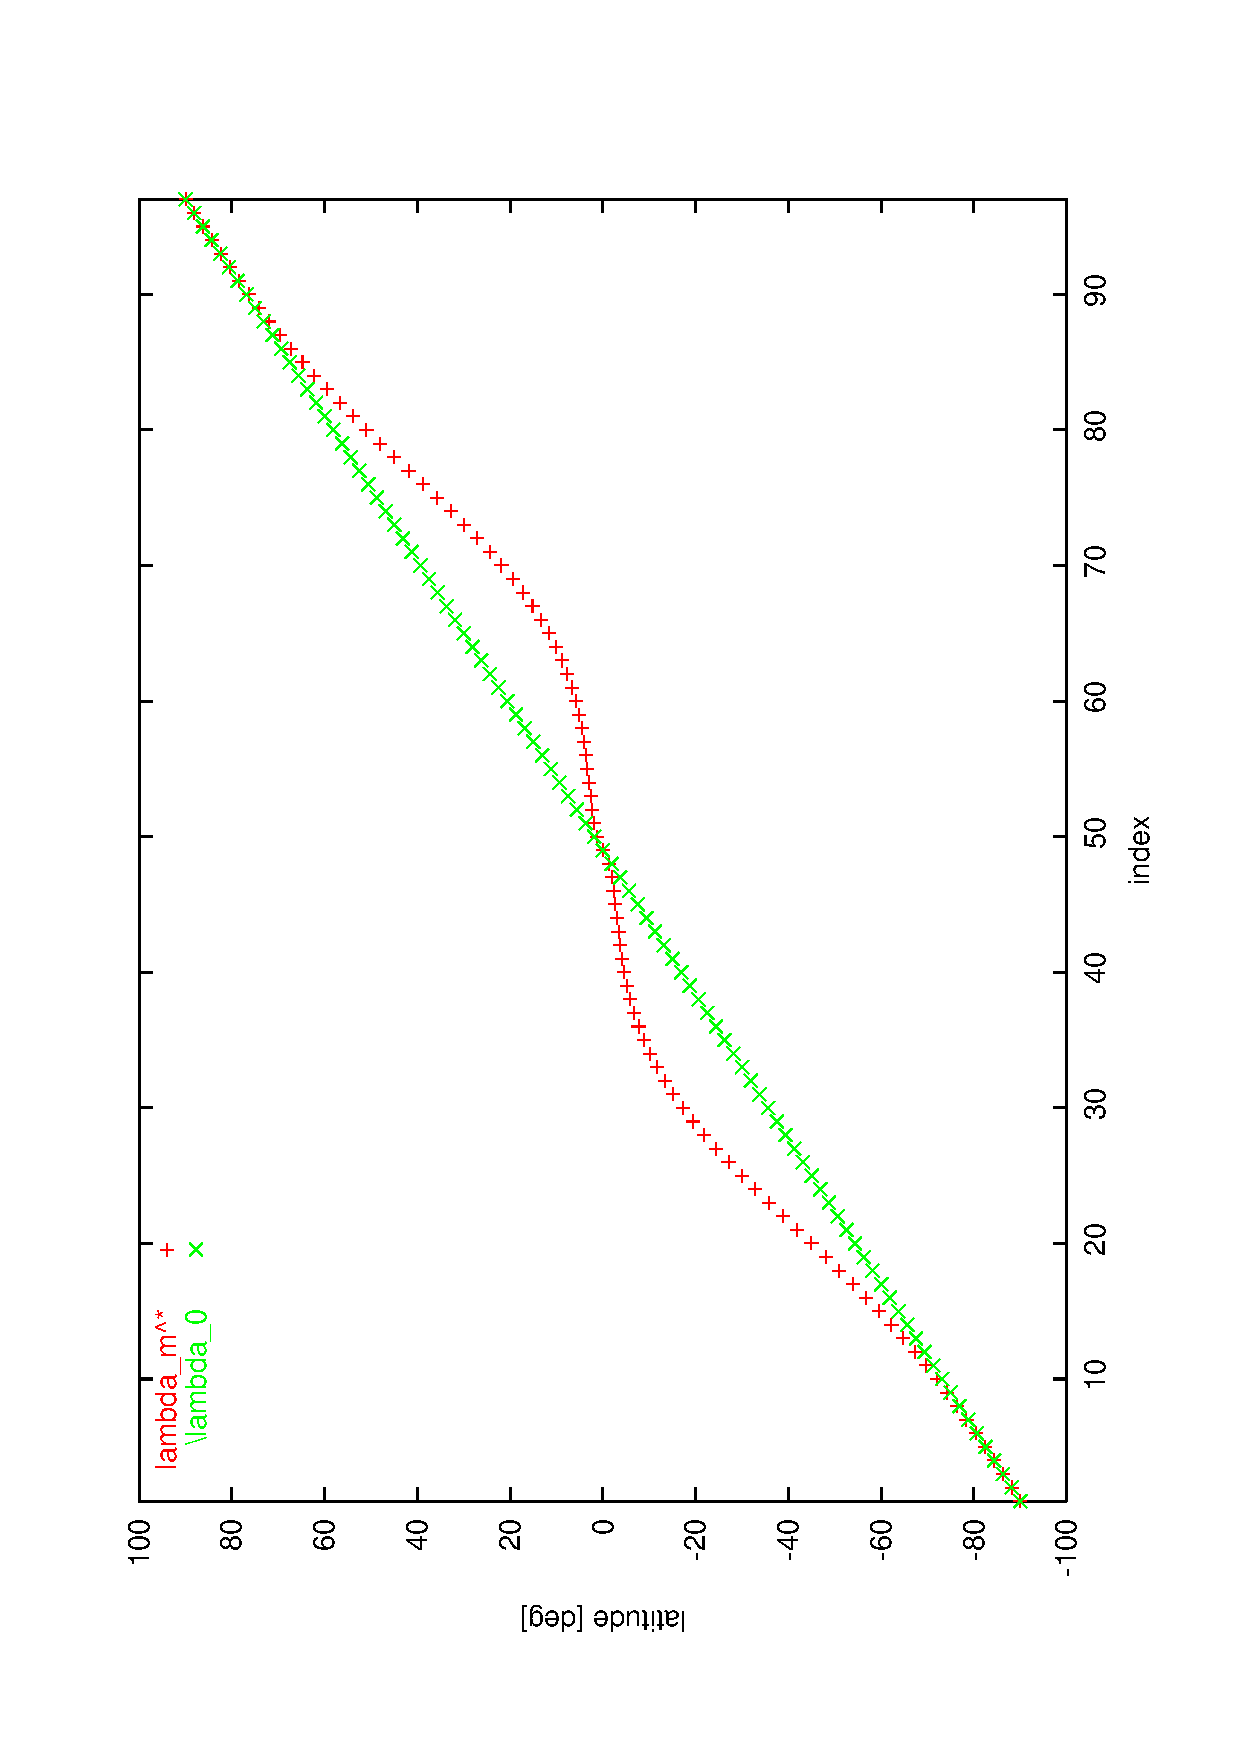
\includegraphics[scale=0.3, angle=-90]{./tex_plot/lambda.epsi}
  \caption{Distribution of modified apex latitude points for $\lambda_0$
  (crosses) and 
  $\lambda_m^*$ (pluses)}
   \label{fig:lambda}
\end{figure}
%
%-------------------------------------------------------------------------------------------
\section{Mapping from and to the geomagnetic grid}
%
The fields in table \ref{tab:map_transf} are mapped from the geographic grid 
to the geomagnetic
grid in \src{subroutine transf}. \src{Subroutine transf} is called from 
\src{subroutine dynamo} once per
timestep.
%
\begin{table}[tb]
\begin{tabular}{|p{3.0cm} ||c|c|c|c|c|c|} \hline
 variable                                  & description            & unit & dimension \\ \hline \hline
%
$\sigma_P$                                 & Pedersen conductivity   & S/m & 3D   \\ 
$\sigma_H$                                 & Hall conductivity       & S/m & 3D   \\
z                                          & geopotential height     & cm & 3D   \\ 
$sin I_m(h_0)$                             & inclination angle       & -  & 2D   \\ 
$B_{e3}(h_0)$                                     & magnetic field component    & T  & 2D   \\
$\frac{\mathbf{d}_1 \cdot \mathbf{d}_2}{D}(h_0)$  & base vector quantity	& - &  2D   \\ 
$\frac{\mathbf{d}_1 \cdot \mathbf{d}_1}{D}(h_0)$  & base vector quantity	& - &  2D   \\
$\frac{\mathbf{d}_2 \cdot \mathbf{d}_2}{D}(h_0)$  & base vector quantity	& - &  2D   \\
${u}_{e1}, {u}_{e2} $                     & neutral wind components & $\frac{m}{s}$ & 3D   \\ \hline
%
\end{tabular}
\caption{Mapped fields in \src{subroutine transf}}
\label{tab:map_transf}
\end{table}  
%
The lower boundary of the TIEGCM model (up to version 1.8) 
is at 97 km, however the field
line integration starts at $h_0=$ 90 km altitude, where the lower boundary 
of the
ionosphere is assumed to lie. Therefore the fields in table \ref{tab:map_transf} 
needed for the field line integration
have to be
extended downward. 
Three additional height levels (k=-2 to 0) are introduced with k being the
height index. The geopotential height $z$ is linearly
extrapolated and the conductivities are assumed to vary exponentially.
%
\begin{alignat}{2}
  z(k)               &= h_0+(k+2)
                \bigl(\frac{z(k=1)-h_0}{3} \bigr) \quad &\text{for k=0 to -2 by -1}  \\
  {\sigma}_{P}(k')  &= {\sigma}_{P}(k'=1)
                exp \bigl(\frac{z(k+\frac{1}{2})-z(k=1\frac{1}{2})}{ fac_{ped}}
		\bigr)\quad &\text{for k' =0 to -2 by -1} \label{eq:condped_ext}   \\
  {\sigma}_{H}(k') &= {\sigma}_{H}(k'=1)
                exp \bigl(\frac{z(k+\frac{1}{2})-z(k=1\frac{1}{2})}{ fac_{hall}}
		\bigr) \quad &\text{for k' =0 to -2 by -1} \label{eq:condhall_ext}   
\end{alignat}
% 
Note that the geopotential height is saved on full pressure levels (k) and 
the conductivities on half pressure levels ($k'=k+\frac{1}{2}$). 
Therefore the geopotential height $z$ for
the conductivity extension (eq. \ref{eq:condped_ext} and 
\ref{eq:condhall_ext}) is calculated at half pressure levels denoted by e.g.
$k'=k+\frac{1}{2}$. The factors at which the conductivities are assumed to decay
below the lower boundary of the model are $fac_{ped}= 5. \times 10^5$ and 
$fac_{hall}= 3. \times 10^5$ \\

The neutral winds $\mathbf{u}$ are assumed to be constant between $h_0$=90 
to 97 km and
can be expressed by
%
\begin{equation}
   \mathbf{u} = \mathbf{e}_1 u_{e1} + \mathbf{e}_2 u_{e2}
\end{equation}
%
with the base vectors $\mathbf{e}_i$  (see \cite{rich95}).
The base vectors $\mathbf{d}_i$ and $\mathbf{e}_i$ satisfy
$\mathbf{d}_i \mathbf{e}_j = \delta_{ij}$ with $\delta_{ij}$ the Kronecker
delta. The components $u_{e1}$
in magnetic eastward and  $u_{e2}$ in down--/equatorward direction at altitude
$h$  are  calculated by 
%
\begin{align}
  u_{e1}(h) &= \mathbf{d}_1(h) \cdot \mathbf{u}(h) \\
  u_{e2}(h) &= \mathbf{d}_2(h) \cdot \mathbf{u}(h)
\end{align}
% 
The height variation of $\mathbf{d}_1(h)$ and $\mathbf{d}_1(h)$ is determined by 
%
\begin{align}
  \mathbf{d}_1(h) &= \bigl[\frac{R_E+h_0}{R_E+h)} \bigr]^{3/2} \mathbf{d}_1(h_0)\label{eq:vary_h_d1} \\
  \mathbf{d}_2(h) &= \bigl[\frac{R_E+h_0}{R_E+h)}\bigr]^{3/2}
      \sqrt{\frac{4.-3. cos^2\lambda_m(h_0)}{(4.-3. \frac{R_E+h_0}{R_E+h} 
      cos^2\lambda_m(h_0)}} \mathbf{d}_2(h_0) \label{eq:vary_h_d2}	    
\end{align}
%
with $\lambda_m(h_0)$ the modified apex value at height $h_0$ which is kept 
constant vertically and thus representing the quasi--dipole latitude.
%
In addition the following quantities are calculated
%
\begin{align}
  \frac{\mathbf{d}_1 \cdot \mathbf{d}_1}{D} \\
  \frac{\mathbf{d}_2 \cdot \mathbf{d}_2}{D} \\
  \frac{\mathbf{d}_1 \cdot \mathbf{d}_2}{D}
\end{align}
% 
These values are calculated at height $h_0$. The values at the pole need special
 treatment
since we have different longitudinal grid points for one spatial point. 
Therefore the pole values are
extrapolated from the longitudinal averaged values next to the pole.
%
\begin{equation}
   x(l_{pole}) = \frac{9 \sum_{lon} x(l_{pole} \pm 1)-\sum_{lon} x(l_{pole} \pm 2)}
      {8 \; nlon}
\end{equation}
%
with the latitudinal index of the pole $l_{pole}$ and $x(l_{pole} \pm 1)$ denoting
the values one grid point off the south-- and northpole respectively. The number of
geographic longitudinal grid points is $nlon$ and $\sum_{lon}$ denotes the sum over all
longitudinal grid points. The following
fields are processed: $z(h)$, $\sigma_P(h)$, ${\sigma}_{H}(h)$, $u_{e1}(h)$, 
$u_{e2}(h)$,
$\frac{\mathbf{d}_1 \cdot \mathbf{d}_1}{D}$, $\frac{\mathbf{d}_2 \cdot \mathbf{d}_2}{D}$, 
$\frac{\mathbf{d}_1 \cdot \mathbf{d}_2}{D}$, $sin I_m$, $B_{e3} $. In addition, periodic
points for these fields are added.

%
The mapping from the geographic to the geomagnetic grid is done for each latitude
separately right before the integration along the field line which foot point at
this latitude. 
The field line integration is described in section 
\ref{cap:fieldlineintg}. The geomagnetic equatorial values 
$\sigma_{P, eq}(h)$, ${\sigma}_{H, eq}(h)$, $u_{e1, eq}(h)$, $u_{e2, eq}(h) $ 
have to be known at each geomagnetic
latitude and therefore are calculated before the field line integration 
is done. The mapping from the geographic to the geomagnetic grid
is done by a  bilinear interpolation. The surrounding geographic grid points
for each geomagnetic grid point and the weighting factors for each of the
geographic points are determined in \src{subroutine apxparm}.


